%% -*- TeX-engine: xetex; ispell-dictionary: "russian" -*-

\documentclass[unicode,mathserif]{beamer}

\newenvironment{stopperenv}{\only{\setbeamercolor{local structure}{fg=red}}}{}

\usepackage{microtype}

\usepackage{amsmath}

\usepackage{mathspec}
\usepackage{xunicode}
\usepackage{xltxtra}
\usepackage{unicode-math}
\defaultfontfeatures{Mapping=tex-text,Ligatures=Common}
\setmainfont{PT Serif}
\setsansfont{PT Sans}
\setmonofont{PT Mono}
\setmathfont{XITS Math}
\newfontfamily\cyrillicfont[Script=Cyrillic]{PT Serif}

\usepackage{polyglossia}
\setdefaultlanguage{russian}
\setotherlanguages{english}

\PassOptionsToPackage{obeyspaces}{url}
\usepackage{hyperref}
\hypersetup{
	colorlinks=true,
    citecolor=darkred
}

\makeatletter
\let\@mycite\@cite
\def\@cite#1#2{{\hypersetup{linkcolor=darkred}[{#1\if@tempswa , #2\fi}]}}
\makeatother

\usepackage{fancyvrb}
\usepackage{chemfig}

\usepackage{tikz}
\usetikzlibrary{arrows,shapes,positioning}

%% Caption hacking.
%% Caption hacking.
\usepackage{subcaption}
\renewcommand{\thesubfigure}{\asbuk{subfigure}}
\renewcommand{\thesubtable}{\asbuk{subtable}}
\usepackage[font=small,tableposition=top,margin=1em]{caption}
\captionsetup{compatibility=false}
\captionsetup[figure]{labelformat=empty}
\captionsetup[table]{labelformat=empty}
\captionsetup[subtable]{labelformat=empty}

\usetheme{Pittsburgh}
\usecolortheme{beaver}
\usefonttheme{professionalfonts}

\setbeamerfont{frametitle}{size=\large}
\setbeamertemplate{footline}[frame number]
\setbeamertemplate{frametitle continuation}{(\insertcontinuationcount)}
\setbeamertemplate{caption}{\insertcaption}
\setbeamertemplate{enumerate items}[default]

\defbeamertemplate{description item}{align left}{\insertdescriptionitem\hfill}

\setbeamercovered{dynamic} % overlays not yet revealed will faintly appear
\beamertemplatenavigationsymbolsempty

\newcommand{\hl}[1]{\textcolor{darkred}{#1}}
\newcommand{\bl}[1]{\textbf{#1}}
\newcommand{\iv}[1]{\setlength{\fboxsep}{0pt}\colorbox{darkred}{\strut \textcolor{white}{#1}}}
\newcommand{\op}[1]{\operatorname{#1}}

\newcommand{\E}[2]{\mathbb{E}_{#1} \left[ #2 \right]}

\newcommand{\theme}[1]{%
  \vspace{28pt}
  \centering\fontsize{40pt}{4em}\selectfont{#1}
}

\begin{document}


\begin{frame}[plain,noframenumbering]
  \title{Моделирование данных бисульфитного секвенирования}
  \author{%
    Сергей Лебедев \\
    Руководитель: О. Ю. Шпынов, науч. сотр. \\
    Рецензент: С. В. Малов, ведущ. науч. сотр., доцент, к.ф.-м. н.}
  \institute{СПбАУ НОЦНТ РАН}
  \date{5 июня 2014 г.}

  \maketitle
\end{frame}


\begin{frame}{Метилирование ДНК}
  \begin{center}
    \begingroup
    \setatomsep{1.8em}
    \chemname[1.8em]{\chemfig[line width=1pt]{*6([,,1]-\chembelow{N}{H}-(=O)-N=(-NH_2)-=)}}{\footnotesize{цитозин}}
    \setchemrel{1pt}{0pt}{8.5em}
    \chemrel[]{->,thick,>=latex'}
    \chemname[1.8em]{\chemfig[line width=1pt]{*6([,,1]-\chembelow{N}{H}-(=O)-N=(-NH_2)-(-\hl{CH_3})=)}}{\footnotesize{5-метилцитозин}}
    \endgroup
  \end{center}

  \begin{itemize}
  \item Цитозин --- один из четырех нуклеотидов, образующих ДНК.
  \item В составе ДНК цитозин может быть <<метилирован>>,
    то есть содержать метильную группу.
  \item Изучение метилирования ДНК важно для понимания механизмов
    дифференцировки клетки и изучения рака.
  \end{itemize}
\end{frame}


\begin{frame}[fragile]{Бисульфитное секвенирование ДНК}
  \begin{Verbatim}[commandchars=\\\{\}, fontsize=\small]
                      m
....C.CC.C.C......CC..\hl{C}.C....  ----+
..........C.CC.........\hl{C}.....      |  бисульфитная
                       m           |  конверсия
                                   |
....U.UU.U.U......UU..\hl{C}.U....  <---+
..........U.UU.........\hl{C}.....  ----+
                                   |
  ..T..    .TT.     ..\hl{C}.           |  секвенирование
 ...T.    T.TG       .\hl{C}.T          |
    T.TT.          T..A            |
            TT..      T.T.     <---+
\end{Verbatim}
\end{frame}


\begin{frame}[fragile]{Представление результатов бисульфитного секвенирования}
  \begin{Verbatim}[commandchars=\\\{\}, fontsize=\small]
                      m
....C.CC.C.C......CC..\hl{C}.C....
..........C.CC.........\hl{C}.....
                       m

  ..T..    .TT.     ..\hl{C}.
 ...T.    T.TG       .\hl{C}.T
    T.TT.          T..A
            TT..      T.T.
                      \iv{↑}
\end{Verbatim}
Возможные представления результатов:
\begin{itemize}
\item пара $(\#C, \#T) = (2, 1)$,
\item уровень метилирования $^{\#C}/_{\#C + \#T} =~^2/_3$,
\item $(\#A, \#T, \#C, \#G) = (1, 1, 2, 0)$.
\end{itemize}
\end{frame}


\begin{frame}{Цель и задачи}
  \begin{block}{}
    Цель --- построить математическую модель, позволяющую анализировать
    результаты бисульфитного секвенирования.
  \end{block}

  \begin{block}{Задачи}
    \begin{itemize}
    \item Проанализировать существующие подходы.
    \item Предложить, обосновать и реализовать несколько вероятностных моделей.
    \item Сформулировать критерии отбора и выбрать наиболее подходящую модель.
    \item Сравнить её с уже существующими.
    \end{itemize}
  \end{block}
\end{frame}


\begin{frame}{Существующие подходы}
  \begin{itemize}
  \item Алгоритм MSC (Methylation Status Calling) разделяет все цитозины на две группы:
    цитозины, содержащие метильную группу, и не содержащие её.
  \item Позволяет контролировать количество ошибок в полученном разделении.
  \item Не учитывает, что
    \begin{itemize}
    \item для метилирования ДНК характерен эффект кластеризации,
    \item секвенаторы делают ошибки при чтении последовательности ДНК.
    \end{itemize}
  \end{itemize}
\end{frame}


\begin{frame}[t]{Предлагаемые модели}
  \begin{enumerate}
  \item Биномиальная \textbf{смесь}:
    \begin{itemize}
    \item моделирует $(\#C, \#T)$ с помощью биномиального распределения;
    \item считает состояния всех цитозинов независимыми.
    \end{itemize}
  \item Биномиальная \textbf{скрытая марковская модель}:
    учитывает зависимость состояний соседних цитозинов.
  \item \textbf{Переключающаяся} биномиальная скрытая марковская модель:
    учитывает геномное расстояние между цитозинами.
  \item Переключающаяся \textbf{мультиномиальная} скрытая марковская модель:
    \begin{itemize}
    \item моделирует $(\#A, \#T, \#C, \#G)$ с помощью мультиномиального распределения;
    \item учитывает наличие ошибок секвенирования.
    \end{itemize}
  \end{enumerate}
\end{frame}


\tikzstyle{state}=[draw, circle, minimum size=2em]
\tikzstyle{obs}=[draw, node distance=6em, fill=gray!60]

\begin{frame}[fragile]{Переключающаяся скрытая марковская модель}
  \centering
  \begin{tikzpicture}[
    node distance=4em,
    every edge/.style={draw,->,thick,>=latex'}]
    \node[obs] (x1) {$(0, 2, 10, 0)$};
    \node[obs, right of=x1] (x2) {$(0, 4, 3, 0)$};
    \node[obs, right of=x2] (x3) {$(1, 5, 0, 1)$};

    \node[state, above of=x1] (s1) {\textbf{?}};
    \node[state, above of=x2] (s2) {\textbf{?}};
    \node[state, above of=x3] (s3) {\textbf{?}};
    \node[node distance=6em, right of=s3] (end) {};
    \path[->] (s1) edge node[above] {$d = 4$} (s2);
    \path[->] (s2) edge node[above] {$d = 1$} (s3);
    \path[->] (s3) edge node[above] {$d = 9$} (end);
    \path[->] (s1) edge (x1);
    \path[->] (s2) edge (x2);
    \path[->] (s3) edge (x3);

    \node[left of=s1] (sl) {состояния};
    \node[below of=x1,node distance=2em] (xl) {наблюдения};
  \end{tikzpicture}
  \begin{itemize}
  \item Скрытые состояния образуют марковский процесс с вероятностями
    перехода, зависящими от расстояния $d$.
  \item Наблюдения $(\#A, \#T, \#C, \#G)$ подчиняются мультиномиальному
    распределению, параметры которого зависят от скрытого состояния.
  \end{itemize}
\end{frame}


\definecolor{brewer red}{rgb}{0.89411,0.10196,0.1098}
\definecolor{brewer blue}{rgb}{0.215686,0.491176,0.7215686}

\begin{frame}[fragile]{Обучение переключающейся скрытой марковской модели}
  \centering
  \begin{tikzpicture}[
    node distance=4em,
    every edge/.style={draw,->,thick,>=latex'}]
    \node[obs] (x1) {$(0, 2, 10, 0)$};
    \node[obs, right of=x1] (x2) {$(0, 4, 3, 0)$};
    \node[obs, right of=x2] (x3) {$(1, 5, 0, 1)$};

    \node[state, above of=x1, fill=brewer red] (s1) {\textbf{M}};
    \node[state, above of=x2, fill=brewer red] (s2) {\textbf{M}};
    \node[state, above of=x3, fill=brewer blue] (s3) {\textbf{U}};
    \node[node distance=6em, right of=s3] (end) {};
    \path[->] (s1) edge node[above] {$d = 4$} (s2);
    \path[->] (s2) edge node[above] {$d = 1$} (s3);
    \path[->] (s3) edge node[above] {$d = 9$} (end);
    \path[->] (s1) edge (x1);
    \path[->] (s2) edge (x2);
    \path[->] (s3) edge (x3);

    \node[left of=s1] (sl) {состояния};
    \node[below of=x1,node distance=2em] (xl) {наблюдения};
  \end{tikzpicture}
  \begin{itemize}
  \item В процессе обучения модели оцениваются вероятности перехода и
    параметры мультиномиального распределения.
  \item У модели два возможных состояния:
    \textbf{M} --- цитозин содержит метильную группы и \textbf{U} --- не содержит её.
  \end{itemize}
\end{frame}


\begin{frame}{Сравнение}
  \begin{table}
    \centering
    \begin{tabular}{lrrr}
      \textbf{Хромосома} & \textbf{MSC} & \textbf{MSHMM} & \textbf{Пересечение} \\
      \noalign{\nobreak\smallskip}
      chr1 & 1136756 & 1291624 & 1136756 \\
      chr2 & 1114488 & 1316179 & 1114488 \\
      chr3 & 896377  & 1040715 & 896377  \\
      $\vdots$ & & &
    \end{tabular}
  \end{table}

  \begin{itemize}
  \item Данные бисульфитного секвенирования стволовых клеток мыши.
  \item В ячейках таблицы --- количество метилированных цитозинов.
  \item Время обучения предлагаемой модели на всех хромосомах генома мыши
    \approx~25~минут.
  \end{itemize}
\end{frame}


\begin{frame}{Пример}
  \begin{figure}
    \centering
    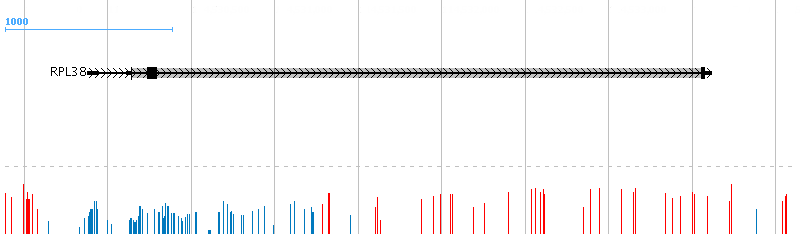
\includegraphics[width=\textwidth]{images/RPL38}
    \caption{Ген <<домашнего хозяйства>> RPL38\footnote{Синий цвет соответствует состоянию \textbf{U},
      красный --- состоянию \textbf{M}.}}
  \end{figure}
\end{frame}


\begin{frame}{Результаты}
  \begin{itemize}
  \item Проведён анализ существующих подходов к моделированию данных бисульфитного
    секвенирования.
  \item Реализованы несколько вероятностных моделей разной степени сложности,
    в качестве итоговой модели выбрана переключающаяся мультиномиальная СММ.
  \item Результаты работы модели согласуются с результатами алгоритма MSC,
    но предлагаемая модель также учитывает:
    \begin{itemize}
    \item зависимость состояний соседних цитозинов в геноме,
    \item наличие ошибок секвенирования.
    \end{itemize}
  \end{itemize}
\end{frame}


\begin{frame}[plain,noframenumbering]
  \begin{block}{Благодарности}
    \begin{itemize}
    \item JetBrains Biolabs
    \item СПбАУ
      \begin{itemize}
      \item Михаил Колмогоров
      \item Павел Яковлев
      \end{itemize}
    \item СПбГУ
      \begin{itemize}
      \item Алексей Кладов
      \item Екатерина Лебедева
      \end{itemize}
    \end{itemize}
  \end{block}

  \begin{block}{Контакты}
    \vspace{7pt}
    \hl{sergei.a.lebedev@gmail.com}
  \end{block}

  \vfill
  \centering
  \Large{Спасибо за внимание!}
\end{frame}


\begin{frame}[plain,noframenumbering]
  \begin{itemize}
  \item Пусть $d_t$ --- количество нуклеотидов в геноме между $(t-1)$-ым и $t$-ым цитозином,
  \item тогда вероятность перехода из состояния $i$ в состояние $j$ на шаге $t$
    $$
    P(s_t = j|s_{t-1} = i, d_t) = \mathbf{A}_{\operatorname{w}(d_t)ij},
    $$
    где $\operatorname{w}(d_t) : \mathbb{N}_0 \to \{1, \ldots, D\}$ --- функция,
    кластеризующая расстояния.
  \item Тогда функция правдоподобия для переключающейся СММ
    $$
    P(\mathbf{x}; \mathbf{\pi}, \mathbf{A}, \mathbf{\theta})
    = \sum\limits_{\mathbf{s} \in \{1, \ldots, S\}^T}
    \pi_{s_1}
    \prod\limits_{t = 2}^T \mathbf{A}_{\operatorname{w}(d_t) s_t s_{t - 1}}
    \prod\limits_{t = 1}^T P(x_t; \theta_{s_t}),
    $$
    где $\mathbf{x} = (x_1, \ldots, x_T)$ --- результаты бисульфитного
    секвенирования, а $\mathbf{s} = (s_1, \ldots, s_T)$ --- скрытые состояния модели.
  \end{itemize}
\end{frame}


\begin{frame}[plain,noframenumbering]
  \begin{table}[ht]
    \centering
    \begin{subtable}[t]{.3\textwidth}
      \centering
      \begin{tabular}{ll}
        0.990 & 0.002 \\
        0.023 & 0.987
      \end{tabular}
      \caption{$\operatorname{w}(d_t) = 1, d_t \in [1, 2]$}
    \end{subtable}\hspace{.025\textwidth}%
    \begin{subtable}[t]{.3\textwidth}
      \centering
      \begin{tabular}{lll}
        0.966 & 0.034 \\
        0.014 & 0.986
      \end{tabular}
      \caption{$\operatorname{w}(d_t) = 5, d_t \in [6, 9]$}
    \end{subtable}\hspace{.025\textwidth}%
    \begin{subtable}[t]{.3\textwidth}
      \centering
      \begin{tabular}{lll}
        0.285 & 0.715 \\
        0.033 & 0.967
      \end{tabular}
      \caption{$\operatorname{w}(d_t) = 9, d_t \ge 118$}
    \end{subtable}
  \end{table}

  \begin{itemize}
  \item Матрицы вероятностей перехода для переключающейся СММ обученной.
  \item Метки столбцов и строчек слева-направо и сверху вниз: \texttt{UNMETHYLATED},
    \texttt{METHYLATED}.
  \item С увеличением расстояния вероятность остаться в том же состоянии
    уменьшается.
  \end{itemize}
\end{frame}


\begin{frame}[plain,noframenumbering]
  \begin{itemize}
  \item FDR (false discovery rate) --- частота ложных предсказаний.
  \item Ограничить количество ошибок можно, контролируя FDR на некотором уровне $\alpha$.
  \item В контексте бисульфитного секвенирования:
    \begin{itemize}
    \item[0] цитозин не содержал метильной группы,
    \item[1] обратное.
    \end{itemize}
  \item При сравнении с алгоритмом MSC FDR контролировался на уровне $\alpha = 0.01$.
  \item Детали процедуры для контроля FDR можно найти в статье
    Cheng, Zhu, <<A classification approach for DNA methylation profiling with bisulfite
    next-generation sequencing data>>, 2014.
  \end{itemize}
\end{frame}

\end{document}
